\subsection{How to Implement Features?}
\begin{frame}{\myframetitle}
	\begin{mycolumns}
		\myexampletight{Given a feature model for graphs \ldots}{
			\centering\featureDiagramGraphs
			%\featureDiagramLegend
		}
		\myexample{\ldots\ we can derive a valid configuration}{
			\small
			\leftmiddleandright{
				$\{G\}$\\
				$\{G,C\}$\\
				$\{G,D\}$\\
				$\{G,C,D\}$\\
			}{
				$\{G,W\}$\\
				$\{G,C,W\}$\\
				$\{G,D,W\}$\\
				$\{G,C,D,W\}$\\
			}{
				$\{G,W,S\}$\\
				$\{G,C,W,S\}$\\
				$\{G,D,W,S\}$\\
				$\{G,C,D,W,S\}$\\
			}
		}
	\mynextcolumn
		\vspace{-10mm}
		\myexampletight{How to Generate Products Automatically?}{
			\centering\foreach \page in {2,12,4,14,6,16,8,18,10,20,42,44}{\includegraphics[width=.23\linewidth,page=\page]{graphs} }
		}
		\mynote{Goals}{
			\begin{itemize}
				\item descriptive specification of a product (i.e., a configuration, a selection of features)
				\item automated generation of a product with compile-time variability
			\end{itemize}
			Focus of the next three lectures \ldots
		}
	\end{mycolumns}
\end{frame}

\subsection{Problems of Ad-Hoc Approaches for Variability}

\subsubsection{Features with Runtime Variability?}
\begin{frame}[fragile]{\myframetitle}
	\footnotesize
	\begin{mycolumns}[animation=none]
\begin{codetight}{}
public class Config {
	~public static boolean COLORED = true;~
	@public static boolean WEIGHTED = false;@
}
\end{codetight}
\begin{codetight}{}
public class Graph {
	...
	Edge add(Node n, Node m) {
		Edge e = new Edge(n, m);
		nodes.add(n); nodes.add(m); edges.add(e);
		@if (Config.WEIGHTED) { e.weight = new Weight(); }@
		return e;
	}
	@Edge add(Node n, Node m, Weight w) {
		if (!Config.WEIGHTED) { throw new RuntimeException(); }
		Edge e = new Edge(n, m);
		nodes.add(n); nodes.add(m); edges.add(e);
		e.weight = w;
		return e;
	}@
	...
}
\end{codetight}
	\mynextcolumn
\begin{codetight}{}
public class Node {
	~Color color;~
	...
	Node(){
		~if (Config.COLORED) { color = new Color(); }~
	}
	void print() {
		~if (Config.COLORED) { Color.setDisplayColor(color); }~
		System.out.print(id);
	}
}
\end{codetight}
\begin{codetight}{}
public class Edge {
	@Weight weight;@
	...
	Edge(Node _a, Node _b) {
		a = _a; b = _b;
		@if (Config.WEIGHTED) { weight = new Weight(); }@
	}
	void print() {
		a.print(); b.print();
		@if (Config.WEIGHTED) { weight.print(); }@
	}
}
\end{codetight}
	\end{mycolumns}
\end{frame}

\begin{frame}{\myframetitle}
	\begin{mycolumns}[widths={40},T]
		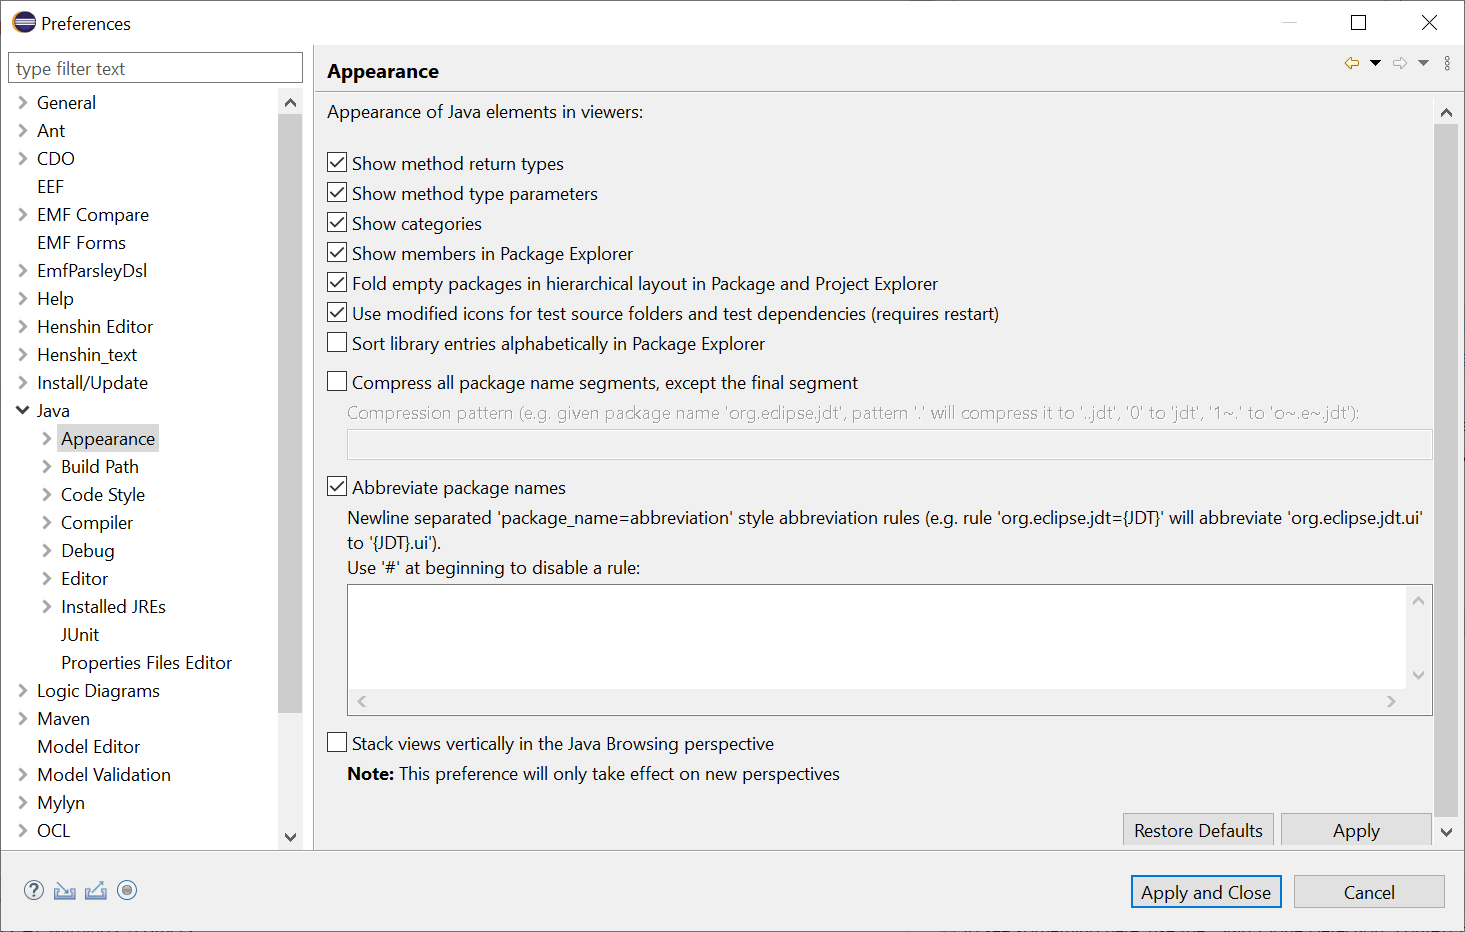
\includegraphics[width=\linewidth]{preferences-eclipse}

		\begin{definition}{How to? -- Preference Dialog}
			\begin{itemize}
				\item implement runtime variability
				\item compile the program
				\item manually adjust preferences based on configuration
				\item run the program
			\end{itemize}
		\end{definition}
	\mynextcolumn
		\leftandright{
			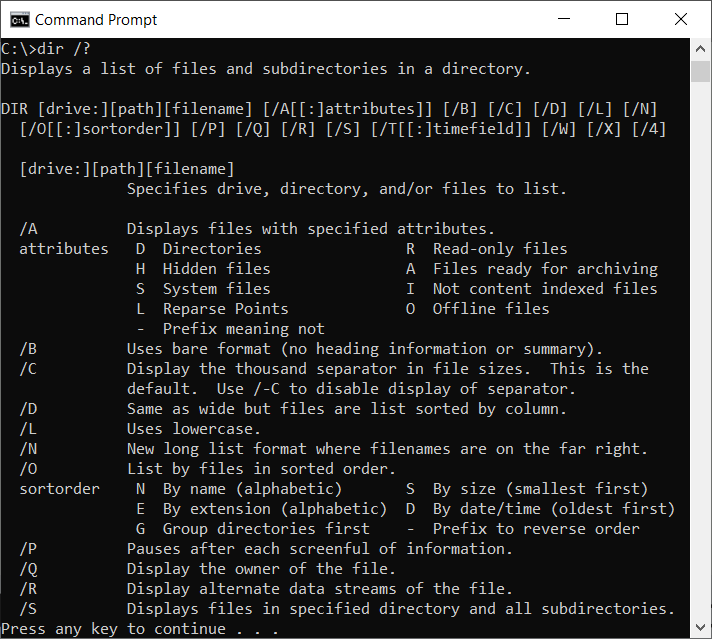
\includegraphics[width=\linewidth]{runtime-parameters-win10-cmd-dir}
		}{
			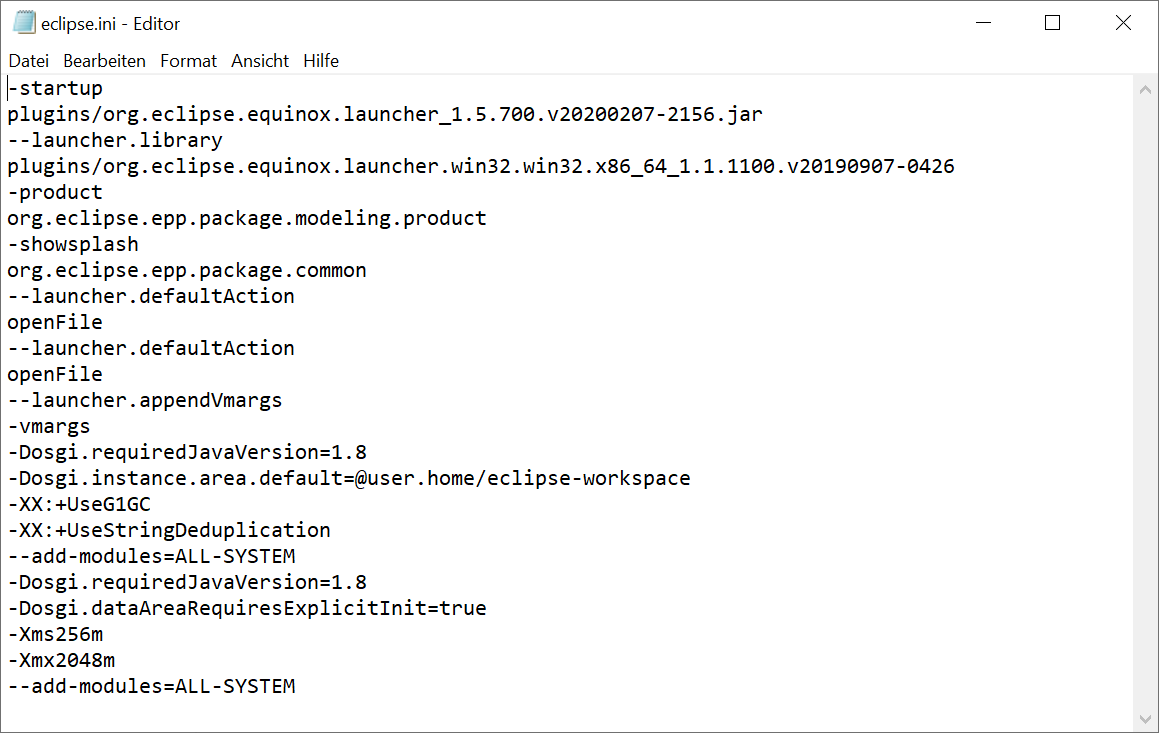
\includegraphics[width=\linewidth]{configfile-eclipse-ini}
		}

		\begin{definition}{How to? -- Command-Line Options / Configuration Files}
			\begin{itemize}
				\item implement runtime variability
				\item compile the program
				\item automatically generate command-line options / configuration files based on configuration
				\item run the program
			\end{itemize}
		\end{definition}
	\end{mycolumns}
\end{frame}

\begin{frame}[fragile]{\myframetitle}
	\begin{mycolumns}[widths={48}]
\begin{codetight}{}
public class Config {
	~public final static boolean COLORED = true;~
	@public final static boolean WEIGHTED = false;@
}
\end{codetight}
		\begin{definition}{How to? -- Immutable Global Variables}
			\begin{itemize}
				\item implement runtime variability
				\item automatically generate class with global variables based on configuration
				\item compile and run the program
			\end{itemize}
		\end{definition}
	\mynextcolumn
		\begin{note}{What is missing?}
			\begin{itemize}
				\item automated generation:\\\hfill for preference dialogs
				\item no compile-time variability / same large binary:\\\hfill for all except immutable global variables
				\item very limited compile-time variability:\\\hfill for immutable global variables
			\end{itemize}
		\end{note}
	\end{mycolumns}
\end{frame}

\subsubsection{Features with Clone-and-Own?}
\begin{frame}{\myframetitle}
	\begin{mycolumns}[widths={30}]
		\centering~

		
\includegraphics[scale=0.2]{alice}
		\includegraphics[scale=0.26,page=2]{graphs}

		
\includegraphics[scale=0.2]{bob}
		\includegraphics[scale=0.26,page=12]{graphs}

		
\includegraphics[scale=0.2]{eve}
		\includegraphics[scale=0.26,page=16]{graphs}
	\mynextcolumn
		\begin{definition}{How to?}
			\begin{itemize}
				\item implement separate project for each product\\(i.e., branch with version control)
				\item download project / checkout branch based on configuration
				\item run build script, if existent
				\item compile and run the program
			\end{itemize}
		\end{definition}
		\begin{note}{What is missing?}
			\begin{itemize}
				\item compile-time variability only for implemented products
				\item no automated generation:\\\hfill for clone-and-own (with version control systems)
				\item automated generation based on build script and extra files:\\\hfill for clone-and-own with build systems
				\item no free feature selection (i.e., configuration)
			\end{itemize}
		\end{note}
	\end{mycolumns}
\end{frame}

\subsection{Introducing Features to Build Systems}
\begin{frame}{\myframetitle}
	\begin{mycolumns}
		\todots
	\mynextcolumn
		\todots
	\end{mycolumns}
\end{frame}

\subsection{KBuild -- The Linux Kernel Build System}
\begin{frame}{\myframetitle}
	\begin{mycolumns}
		\todots
	\mynextcolumn
		\todots
	\end{mycolumns}
\end{frame}
% https://docs.kernel.org/kbuild/kbuild.html

\subsection{Discussion of Features with Build Systems}
\begin{frame}{\myframetitle}
	\begin{mycolumns}
		\todots
	\mynextcolumn
		\todots
	\end{mycolumns}
\end{frame}
